% !TEX root = omar-thesis-proposal.tex
\section{Introduction}\begin{figure}
\begin{center}
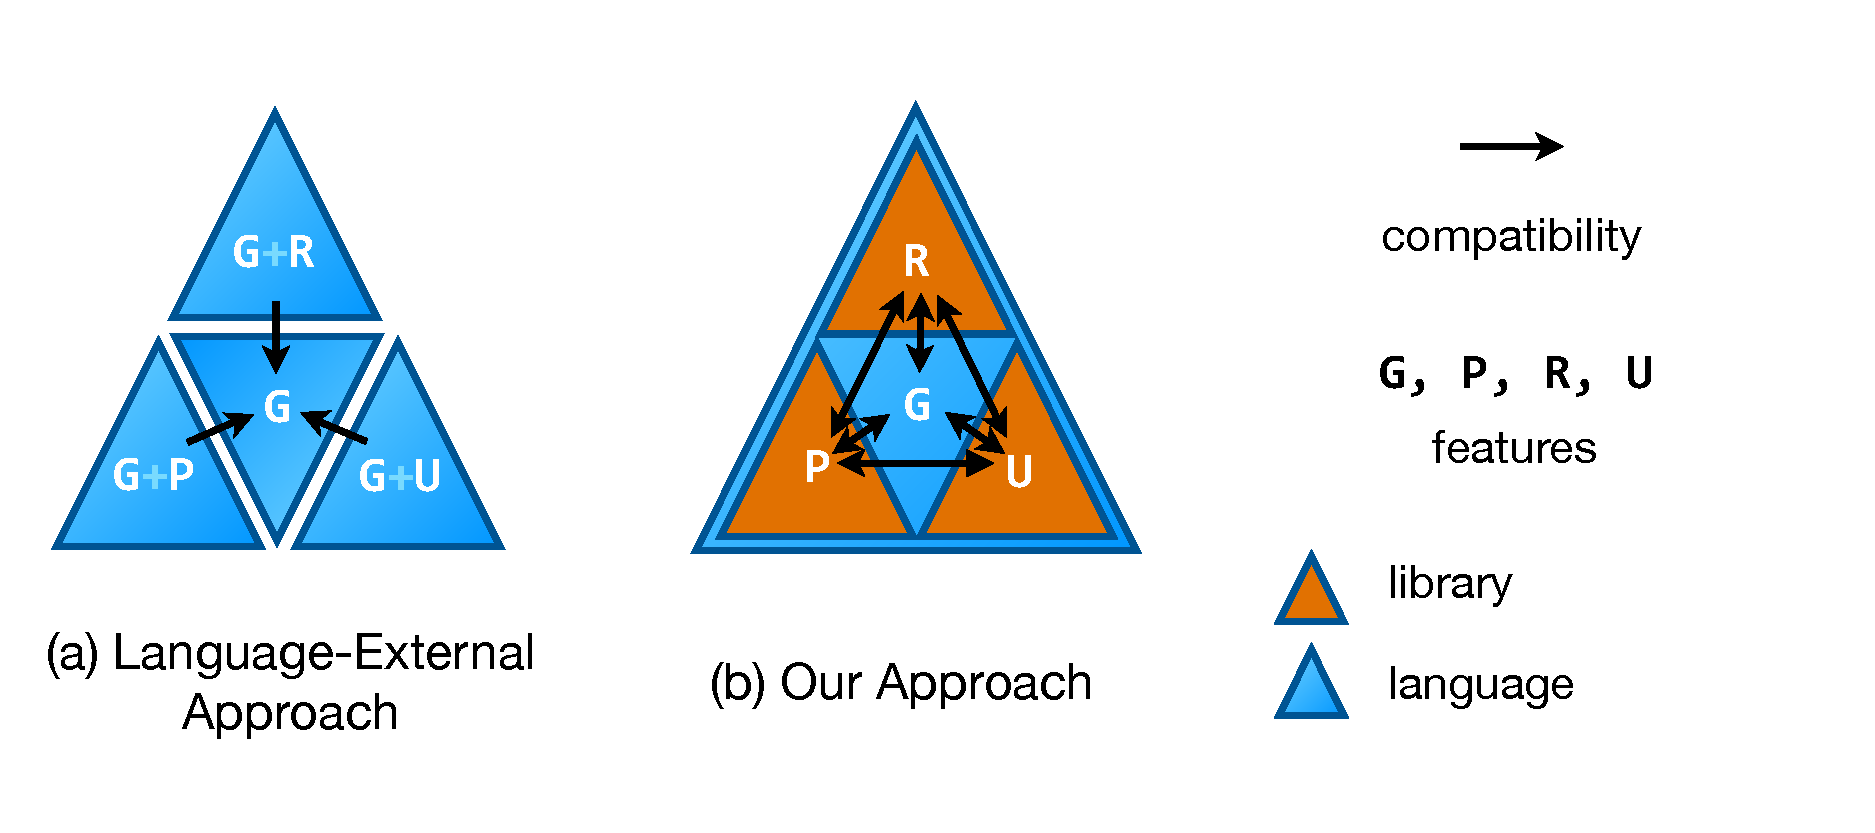
\includegraphics[scale=0.45]{approaches.pdf}
\end{center}
\vspace{-20px}
\caption{\small (a) With the language-external approach, novel constructs are packaged into separate languages. Users can only safely and naturally call into languages if the interface uses common constructs and an interoperability layer has been developed (the \emph{interoperability problem}). (b) With the language-internal approach, there is one extensible host language and the compile-time and edit-time logic governing novel constructs is expressed within libraries. If the extension mechanism guarantees the safety of arbitrary compositions of extensions, the necessary primitives can simply be imported by library clients as needed, and so interoperability is not a problem.}
\label{approaches}
\end{figure}
Designing and implementing a programming language together with its supporting tools (collectively, a \emph{programming system}) that has a sound theoretical foundation, helps users identify and fix errors as early as possible, supports a natural programming style, and that performs well across diverse problem domains and hardware platforms remains a grand challenge in computing. No small, fixed collection of primitive abstractions and tools has been found to fully satisfy these criteria in all situations. Rather, researchers and domain experts  continue to design and implement novel abstractions, provide alternative implementations of existing abstractions, and supplement languages with new tools in order to better satisfy these criteria within the constraints of different problem domains.

To realize a new abstraction or system behavior, such experts can choose either a \emph{language-internal approach}, where they work within an existing language and distribute their solutions as libraries, or a \emph{language-external approach}, where they either derive a new programming system or extend an existing system by some mechanism that is not part of the language itself, such as an extension mechanism supported by a {particular} compiler, editor or other tool.

When possible, taking the \emph{language-internal approach} is significantly simpler and more practical. If an abstraction or system behavior can be realized by creatively repurposing existing language constructs, then  providers and clients face fewer barriers to adoption. % -- library-based constructs cannot interfere with one another (assuming a suitable namespacing standard), libraries benefit from common distribution infrastructure and tool support, and externally-accessible library interfaces need not be restricted to a fixed common subset of all available constructs (e.g. the object system of the JVM or CLI).  We diagram this key latter distinction in Figure \ref{approaches}. 
Unfortunately, this is very often \emph{not} possible today because from the perspective of library code, the programming system is a largely inflexible, \emph{monolithic} entity. That is, the language's syntax and its static and dynamic semantics are fixed in advance, the compiler is a ``black box'' implementation of these fixed semantics, and other tools operate according to domain-agnostic protocols that use only the basic structure of the program as input. To supplement any of these components of the programming system, experts must step out of the language, and often out of the programming system entirely. 

In these situations, experts must take a \emph{language-external approach}, often by developing and distributing new constructs together with a new language and developing an array of necessary tools. This increases the development burden on these experts, although tools like compiler generators and language workbenches have started to simplify this process, and also requires experts to couple their innovations with a collection of other unrelated design choices, making adoption more difficult for clients. 

A more fundamental limitation of the language-external approach arises at the interface between languages. The specialized constructs particular to one language cannot always be safely and naturally expressed in another, so building a program out of components written in different languages, when such constructs are used at the interface boundaries, can be difficult. We refer to this as the \emph{interoperability problem}. One increasingly common strategy taken by language designers to partially address the interoperability problem is to target an established language and runtime, such as the Java Virtual Machine (JVM), and support a superset of its features. Scala \cite{scala} and F\# \cite{fsharp} are examples of languages that have taken this approach. This addresses interoperability in only one direction (Figure \ref{approaches}a). While calling into the common language becomes straightforward, calls in the other direction, or between languages sharing the common target, are still restricted by the constructs available in the common language. If interoperability in both directions is desired, the new languages must only include constructs that can be expressed safely and naturally in the target language. More novel innovations, however, are often difficult to define in terms of familiar forms in ways that guarantee all necessary invariants are maintained and that are reasonably natural for users of other languages. In F\#, for example, the type system guarantees that null values cannot occur, but this invariant is not maintained when calling from other languages. The F\# type system also includes support for units of measure \cite{fsharpunits}, but such domain-specific invariants cannot be guaranteed when calling into F\# from other CLI languages. Similarly, interfaces built using Scala traits can be difficult to implement from Java or other JVM languages. In some cases, features are omitted entirely due to this requirement. For example, the module system in F\# is significantly limited relative to the module system in its predecessor, OCaml, due to the need for bidirectional interoperability between other languages on the common language infrastructure (CLI). 

For these reasons, we argue that language-external approaches should be considered harmful. The goal of the research proposed here is to fundamentally reorganize the core components of the programming system so that such language-external approaches are less frequently necessary, by designing \emph{language-internal} mechanisms that give developers control, from within the language itself, over edit-time and compile-time behaviors that are currently centrally controlled by language and tool designers and design committees\footnote{To be a bit piquant, one might compare today's monolithic programming languages to isolationist {centrally-planned} economies, whereas extensible languages more closely resemble modern market economies. We leave fleshing out such analogies to the reader.}. In particular, we will describe how parsing, typechecking, translation and code completion can all be influenced by user-defined constructs \todo{describe what this looks like - libraries + reference Fig 1b.} in ways that preserve the safety of the language as a whole and admit strong composition principles \todo{elaborate on safety requirements, merge with next paragraph}.

The extension mechanism must be expressive enough to allow users to associate rich run-time, compile-time and edit-time behaviors with user constructs directly, while being sufficiently restrictive to maintain the global safety properties of the language and system as a whole, and to ensure that constructs cannot interfere with one another. This explicit consideration of the full programming system, and the tension between expressiveness and safety, are key aspects of our approach.
